\documentclass[submit]{harvardml}

\course{CS181-S24}
\assignment{Assignment \#4}
\duedate{11:59pm March 29, 2024}

\usepackage[OT1]{fontenc}
\usepackage[colorlinks,citecolor=blue,urlcolor=blue]{hyperref}
\usepackage[pdftex]{graphicx}
\usepackage{graphicx}
\usepackage{caption}
\usepackage{fullpage}
\usepackage{soul}
\usepackage{amsmath}
\usepackage{amssymb}
\usepackage{framed}
\usepackage{color}
\usepackage{todonotes}
\usepackage{listings}
\usepackage{common}

\usepackage[mmddyyyy,hhmmss]{datetime}

\definecolor{verbgray}{gray}{0.9}

\lstnewenvironment{csv}{
  \lstset{backgroundcolor=\color{verbgray},
  frame=single,
  framerule=0pt,
  basicstyle=\ttfamily,
  columns=fullflexible}}{}
 
\begin{document}

\begin{center}
{\Large Homework 4: SVM, Clustering, and In-Depth Ethics}\\
\end{center}

\subsection*{Introduction}

This homework assignment will have you work with SVMs, clustering, and engage with the ethics lecture.

\subsection*{Resources and Submission Instructions}
We encourage you to
read Chapter 5 in the textbook to learn more about SVMs, 6.2 to review k-means clustering, and 6.3 to review HAC.

Please submit the \textbf{writeup PDF to the Gradescope assignment `HW4'}. Remember to assign pages for each question.

Please submit your \textbf{\LaTeX\ file and code files to the Gradescope assignment `HW4 - Supplemental'}. 

You can use a \textbf{maximum of 2 late days} on this assignment.  Late days will be counted based on the latest of your submissions. 

\newpage

%%%%%%%%%%%%%%%%%%%%%%%%%%%%%%%%%%%%%%%%%%%%%
% Problem 1
%%%%%%%%%%%%%%%%%%%%%%%%%%%%%%%%%%%%%%%%%%%%%
\begin{problem}[Fitting an SVM by hand, 10pts]

  For this problem you will solve an SVM by hand, relying on principled rules and SVM properties. 
  For making plots, however, you are allowed to use a computer or other graphical tools.

Consider a dataset with the following 7 data points each with $x \in \reals$ and $y \in \{ -1, +1 \}$ : \[\{(x_i, y_i)\}_{i = 1}^7 =\{(-3 , +1) , (-2 , +1 ) , (-1,  -1 ), (0, +1), ( 1 , -1 ), ( 2 , +1 ) , (3 , +1 )\}\] Consider
mapping these points to $2$ dimensions using the feature vector $\bphi(x) =  (x, -\frac{8}{3}x^2 + \frac{2}{3}x^4 )$. The hard margin classifier training problem is:
%
\begin{align*}
  &\min_{\mathbf{w}, w_0} \frac{1}{2}\|\mathbf{w}\|_2^2 \label{eq:dcp} \\
  \quad \text{s.t.} \quad & y_i(\mathbf{w}^\top \bphi(x_i) + w_0) \geq 1,~\forall i \in \{1,\ldots, n\}\notag
\end{align*}

Make sure to follow the logical structure of
the questions below when composing your answers, and to justify each step.

\begin{enumerate}
\item Plot the transformed training data in $\reals^2$ and draw the optimal decision boundary
of the max margin classifier. You can determine this by inspection (i.e. by hand, without actually doing any calculations).

\item  What is the value of the margin achieved by the optimal
decision boundary found in Part 1? 

\item Identify a unit vector that is orthogonal to the decision boundary.

\item Considering the discriminant $h(\bphi(x);\boldw,w_0)=\boldw^\top\bphi(x) +w_0$, 
give an expression for {\em all possible} $(\boldw,w_0)$ that define
the decision boundary. Justify your answer.

  \item Consider now the training problem for this dataset. Using your answers so far,
    what particular solution to $\boldw$ will be optimal for the
    optimization problem?

  \item What is the corresponding optimal value of $w_0$ for the $\boldw$ found in Part 5 (use your result from Part 4 as guidance)? Substitute in these optimal values and write out the discriminant function
    $h(\bphi(x);\boldw,w_0)$ in terms of the variable $x$ .


\item Which points could possibly be support vectors of the classifier?  Confirm that
  your solution in Part 6 makes the constraints above tight---that is,
  met with equality---for these candidate points.

\item Suppose that we had decided to use a different feature mapping
    $\bphi'(x) = (x, -\frac{31}{12}x^2 + \frac{7}{12}x^4 )$.  Does
    this feature mapping still admit a separable solution?  How does
    its margin compare to the margin in the previous parts?  Based on
    this, which set of features might you prefer and why? 
    
\end{enumerate}

\end{problem}

\subsection*{Solution}

\newpage


1. 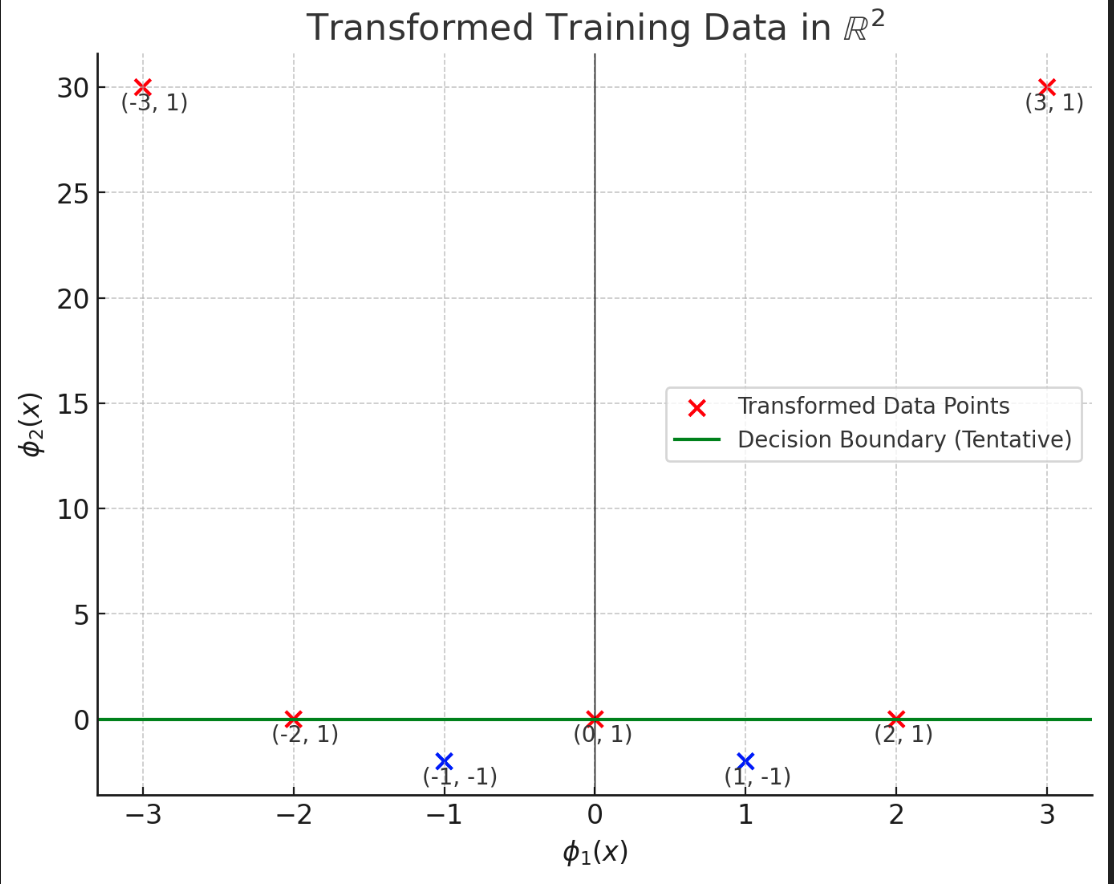
\includegraphics[width=0.5\linewidth]{hw4/11.png}\\ The original data is linearly separable with each positive-class point above $x_2 = 0$ and negative-class point lie on $x_2 = -2$. The margin is maximized when the decision boundary is $x_2 = -1$, making the positive hyperplane is $x_2 = 0$ with the data points $(-2, +1)$, $(0, +1)$, $(2, +1)$ as support vectors, and the negative hyperplane is $x_2 = -2$ with the data points $(-1, -1)$, $(1, -1)$ as support vectors. Translations would reduce the margin from the positive and negative planes while rotations would shrink the support vectors and reduce the margins. \\
2. To find the value of the margin, I take the perpendicular distance from any of the 3 positive-class data points $(-2, +1)$, $(0, +1)$, $(2, +1)$ or any of the 2 negative-class data points $(-1, -1)$, $(1, +1)$. This makes it 1. \\
3. $\mathbf{w} = [0, 1]^T$\\
4. $x_2 = -1$. I know the points $x_2 > -1$ should be positively classified and all points with $x_2 < -1$ should be negatively classified, meaning the set of all possible $(\mathbf{w}, w_0)$ is $\{ (t[0, 1]^T, t) \,|\, t \in \mathbb{R}^+ \}$. The boundary for $(x_1, -1)$  should satisfy $\mathbf{w}^T[x_1, -1]^T + w_0 = 0$ for all $x_1 \in \mathbb{R}$ or $w_1x_1 - w_2 + w_0 = 0\forall x_1 \in \mathbb{R}$.  \\
5. \(w = [0, 1]^T\). The objective function is minimizing \(w\) when we defined the optimal decision boundary as \(\{((0, w_0)^T, w) \,|\, w \in \mathbb{R}^+\}\). In other words, we are constrained by 

    \[
    \begin{cases}
        +1(30w + w) \geq 1 & \Rightarrow w \geq \frac{1}{31} \\
        +1(0w + w) \geq 1 & \Rightarrow w \geq 1 \\
        -1(-2w + w) \geq 1 & \Rightarrow w \geq 1
    \end{cases}
    \] \\
6.  Combining our previous solutions, \(w_0 = 1\). This makes the discriminant function: 
    \[
    h(\boldsymbol{\phi}(x); \mathbf{w}, w_0) = \mathbf{w}^T(\boldsymbol{\phi}(x)) + w_0 = -\frac{8}{3}x_2 + \frac{2}{3}x_2^4 + 1
    \] \\
7. The discriminant function for the 5 aforementioned points on the positive and negative hyper planes is \(1, 1, 1, -1, -1\). The constraints bind with equality when the three support vectors on the positive hyperplane are \(y_ih(\boldsymbol{\phi}(x_i)) = -1 \cdot 1 = -1\) and the two on the negative are \(= -1 \cdot -1 = 1\). \\
8. The new feature mapping $\boldsymbol{\phi}'(x) = (x, -\frac{31}{12}x^2 + \frac{7}{12}x^4)$ maintains separability as it keeps the sign consistency between classes after transformation. Since the margin is inversely proportional to the norm of $\mathbf{w}$, the comparison between the original and new margin depends on the spread of the transformed data in the feature space. This answer is dependent on whether separability is retained, but assuming it is the mapping with the larger margin would typically be preferred due to better generalization ability. The preference for $\boldsymbol{\phi}$ or $\boldsymbol{\phi}'$ hinges on which mapping yields a larger margin, as larger margins generally correlate with more robustness.




%%%%%%%%%%%%%%%%%%%%%%%%%%%%%%%%%%%%%%%%%%%%%
% Problem 2
%%%%%%%%%%%%%%%%%%%%%%%%%%%%%%%%%%%%%%%%%%%

\begin{problem}[K-Means and HAC, 20pts]

For this problem you will implement K-Means and HAC from scratch to cluster image data. You may use \texttt{numpy} but no third-party ML implementations (eg. \texttt{scikit-learn}).

Your job is to implement K-means and HAC on MNIST, the collection of handwritten digits that you saw in HW3, and to test whether these relatively
simple algorithms can cluster similar-looking images together.

The code in \texttt{homework4.ipynb} loads the images into your environment into two arrays -- \texttt{large\_dataset}, a 5000x784 array, will be used for K-means, while \texttt{small\_dataset}, a 300x784 array, will be used for HAC. In your code, you should use the $\ell_2$ norm (i.e. Euclidean distance) as your distance metric.

\textbf{Important:} Remember to include all of your plots in your PDF submission!

% \textbf{Checking your algorithms:} Instead of an Autograder file, we have provided a similar dataset, \texttt{P2\_Autograder\_Data}, and some visualizations, \texttt{HAC\_visual} and \texttt{KMeans\_visual}, for how K-means and HAC perform on this data. Run your K-means (with $K=10$ and \texttt{np.random.seed(2)}) and HAC on this second dataset to confirm your answers against the provided visualizations. Do \textbf{not} submit the outputs generated from \texttt{P2\_Autograder\_Data}. Load this data with \texttt{data = np.load(`P2\_Autograder\_Data.npy')}.

\begin{enumerate}

\item Starting at a random initialization and $K = 10$, plot the
  K-means objective function (the residual sum of squares) as a
  function of iterations and verify that it never increases.

\item For $K=10$ and for 3 random restarts, print the mean image (aka
  the centroid) for each cluster. There should be 30 total images.

\item Repeat Part 2, but before running K-means, standardize or center
  the data such that each pixel has mean 0 and variance 1 (for any
  pixels with zero variance, simply divide by 1). For $K=10$ and 3
  random restarts, show the mean image (centroid) for each
  cluster. Again, present the 30 total images in a single
  plot. Compare to Part 2: How do the centroids visually differ? Why?

\item Implement HAC for min, max, and centroid-based linkages. Fit
  these models to the \texttt{small\_dataset}.  For each of these 3
  linkage criteria, find the mean image for each cluster when using
  $10$ clusters. Display these images (30 total) on a single plot.

  How do the ``crispness'' of the cluster means and the digits
  represented compare to mean images for k-means?  
  Why do we only ask you to run HAC once?  

  \textbf{Important Note:} For this part ONLY, you may use
  \texttt{scipy}'s \texttt{cdist} function to calculate Euclidean
  distances between every pair of points in two arrays.

\item For each of the HAC linkages, as well as one of the runs of your
  k-means, make a plot of ``Number of images in cluster" (y-axis)
  v. ``Cluster index" (x-axis) reflecting the assignments during the
  phase of the algorithm when there were $K=10$ clusters.

  Intuitively, what do these plots tell you about the difference
  between the clusters produced by the max and min linkage criteria?

  Going back to the previous part: How does this help explain the
  crispness and blurriness of some of the clusters?  

\end{enumerate}
\end{problem}

\newpage
\begin{framed}
\noindent\textbf{Problem 2} (cont.)\\
\begin{enumerate}
\setcounter{enumi}{5}
\item For your K-means with $K = 10$ model and HAC min/max/centroid
  models using $10$ clusters on the \texttt{small\_dataset} images,
  use the \texttt{seaborn} module's \texttt{heatmap} function to plot
  a confusion matrix between each pair of clustering methods.  This
  will produce 6 matrices, one per pair of methods. The cell at the
  $i$th row, $j$th column of your confusion matrix is the number of
  times that an image with the cluster label $j$ of one method has
  cluster $i$ in the second method.  Which HAC is closest to k-means?
  Why might that be?


\item Let's return to the postal service example from HW3.  Do you
  think that clustering is a good way to identify digits, that is,
  first cluster the data, and then, for any new data point, classify
  it based on its cluster?
  \begin{enumerate}
\item In particular, do you expect the clusters to correspond with the
  true labels?  Is that a good way to evaluate clustering?
\item In the context of adversaries, how might clusterings be
  attacked?  How is the process similar or different to the process
  for attacking classification models (like kNN and the generative classifiers that we saw in HW2)?
\end{enumerate}
  
\end{enumerate}
\end{framed}


\subsection*{Solution}

%qwer 
\newpage
1. Plot: 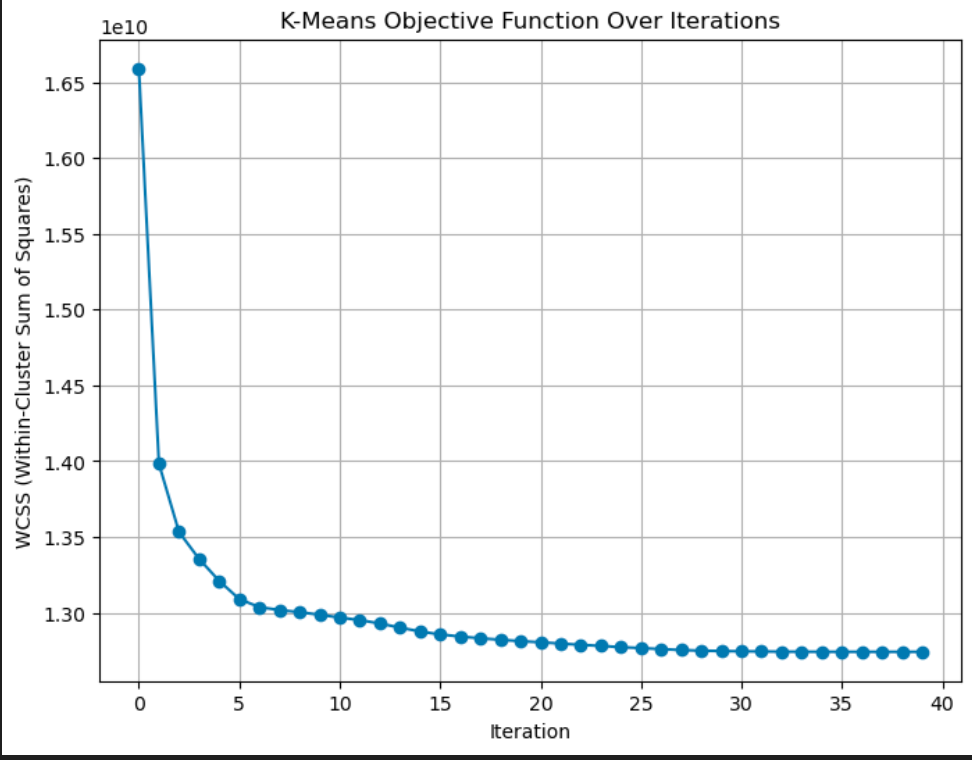
\includegraphics[width=0.5\linewidth]{hw4/21.png}\\
2. Image 1: 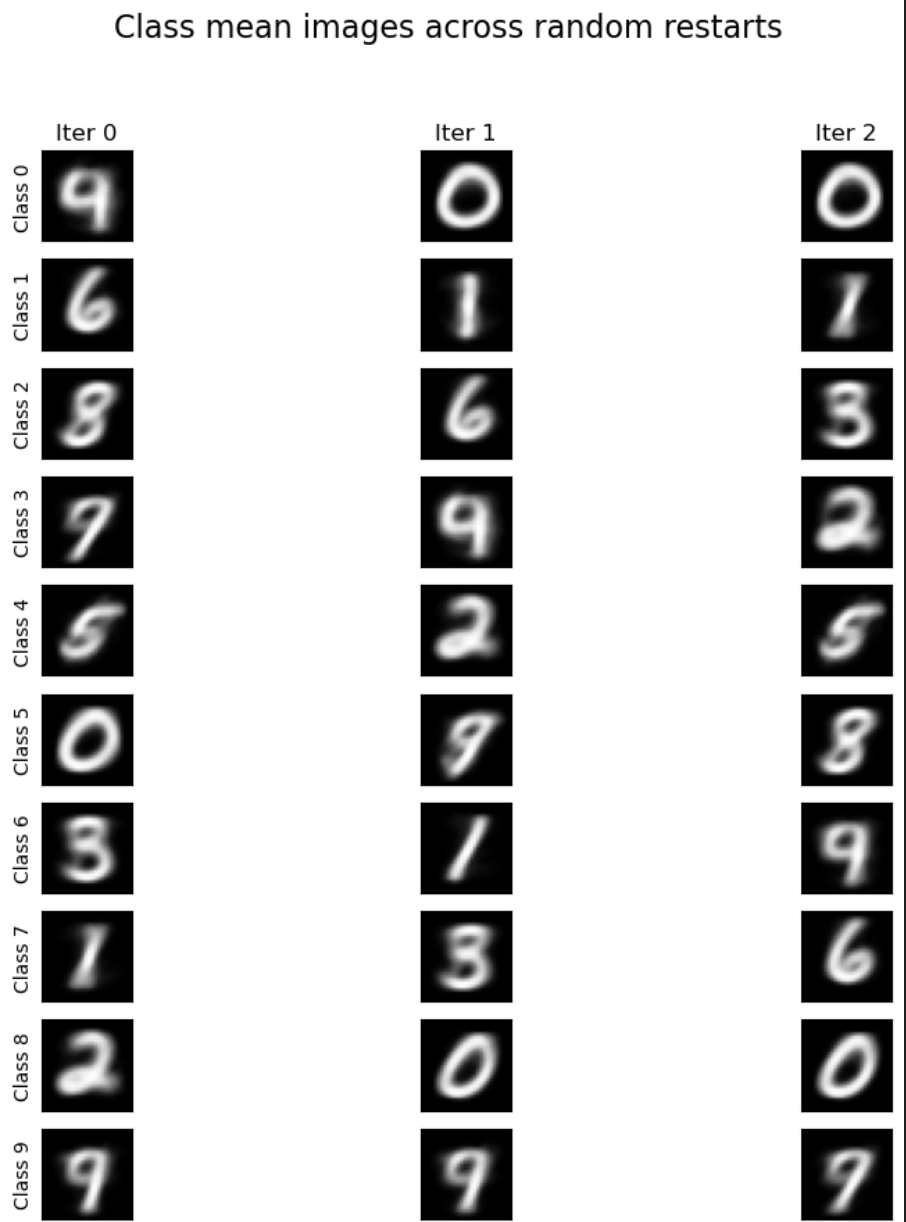
\includegraphics[width=0.5\linewidth]{hw4/22.png}\\
3. Image 2: 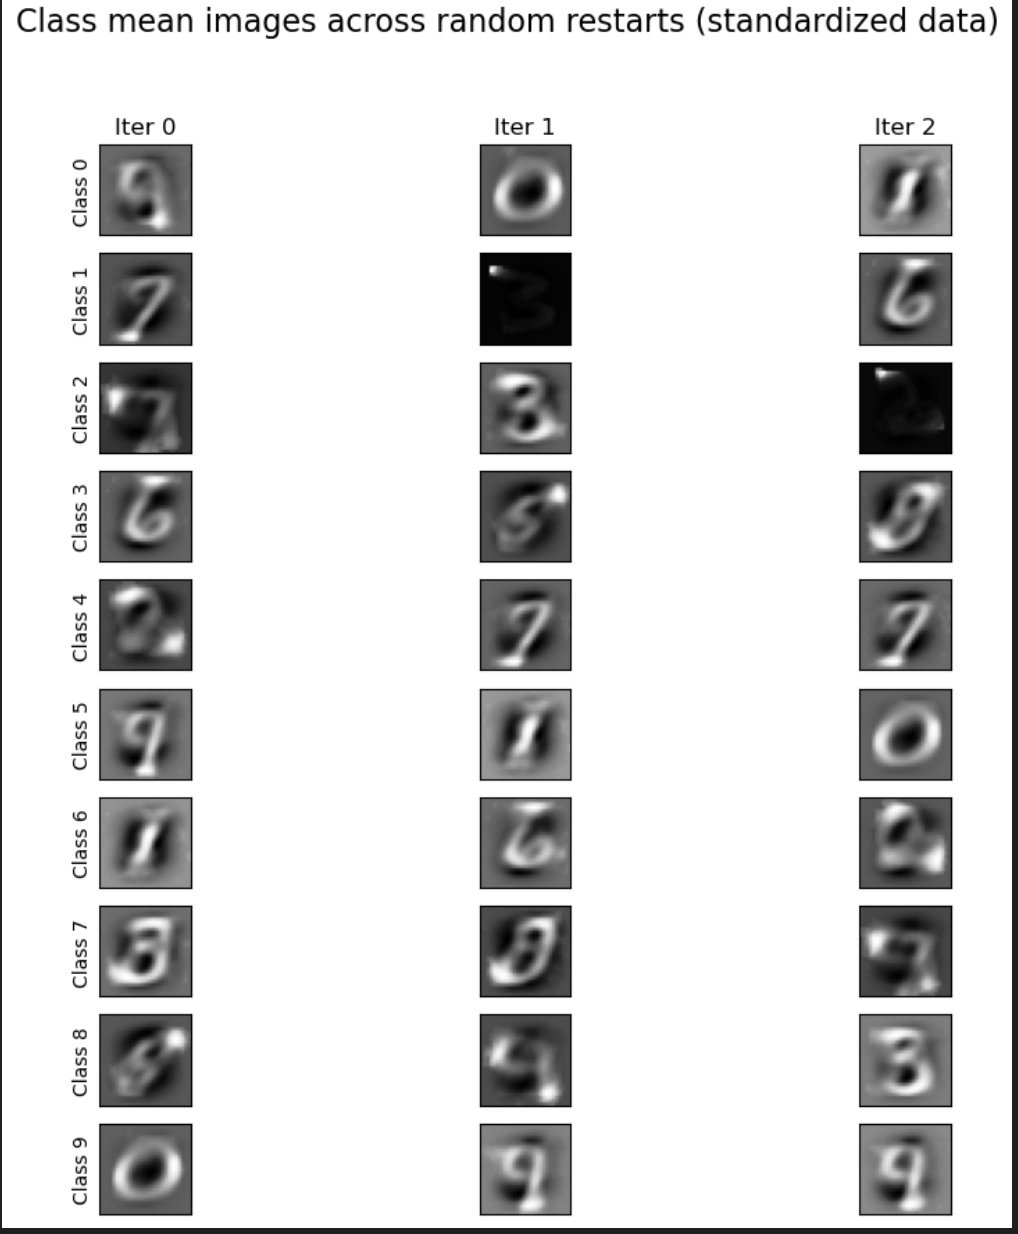
\includegraphics[width=0.5\linewidth]{hw4/23.png}\\
The centroids from the K-means clustering in Part 3 are less defined than those in Part 2 largely because standardization provides an equal weight to all of the pixels irrespective of their initial variability. Pixels that lower influence (variance) now equally contribute to the calculation, which yields centroids that show the how digits are common more diffusely. \\
4. Image 3: 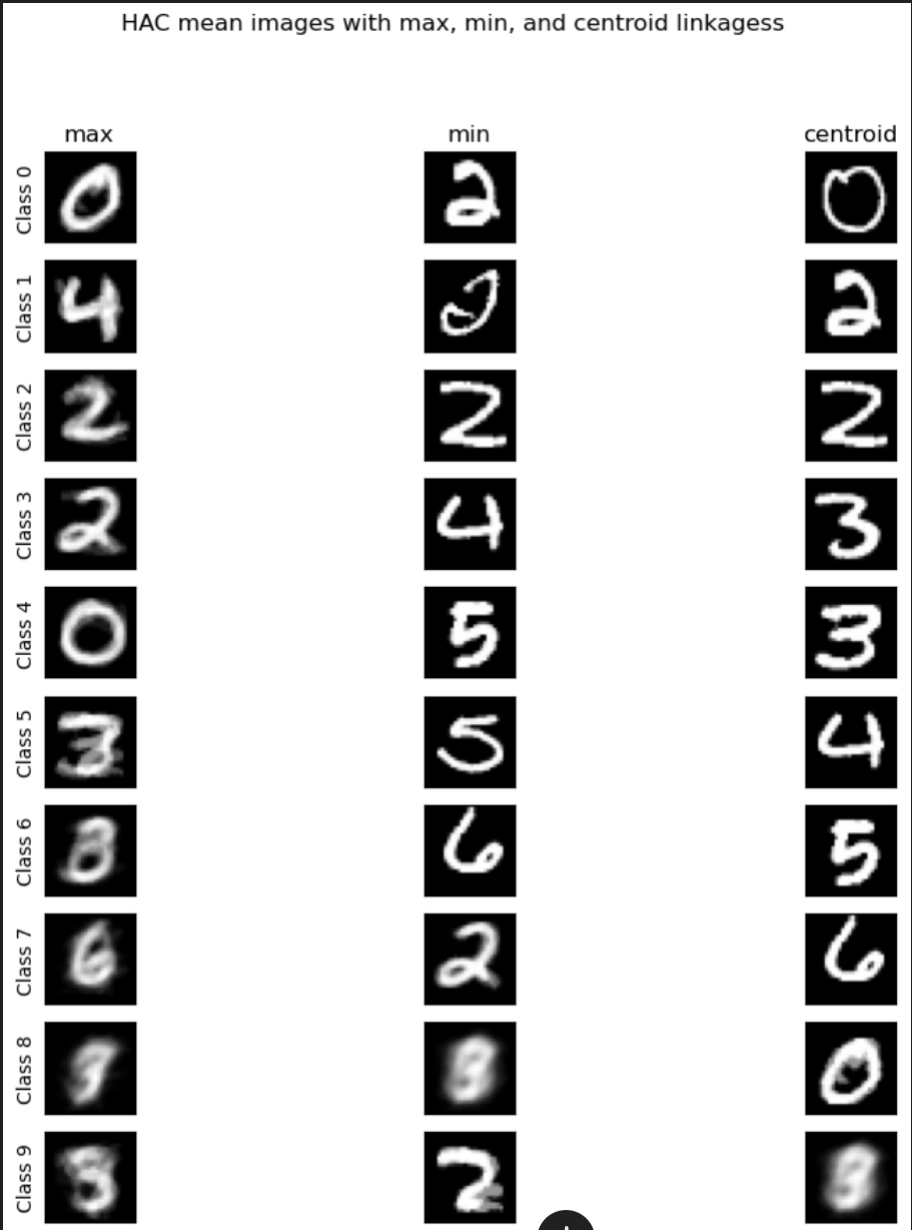
\includegraphics[width=0.5\linewidth]{hw4/24.png}\\
THE HAC cluster are less crisp because the hierarchical nature of the program doesn't properly optimize for within-cluster variance, resulting in potentially more blurred means. HAC was run only once and the fact that it deterministically produce the same clusters from a given initial state, whereas K-means is non-deterministic due to random initialization and can yield different results across runs, shows it requires multiple restarts to find a 'more reasonable' local min. \\
5. The plots show that max linkage tends to produce more balanced cluster sizes, whereas min linkage results in one disproportionately large cluster and several much smaller ones. Max linkage merges clusters based on the farthest pair of points, leading to more cohesive and similarly-sized clusters, which might help maintain the distinctness or "crispness" of the digit representations. Min linkage, on the other hand, merges the closest pair of points, which can result in one cluster aggregating most of the data points early on, leading to a large, less distinct cluster where the mean can be blurred due to the diverse range of digits being combined. This large variance within the min linkage's dominant cluster can explain the blurriness observed, as the mean image represents a wider range of digits. \\
6. Image 4,5,6: 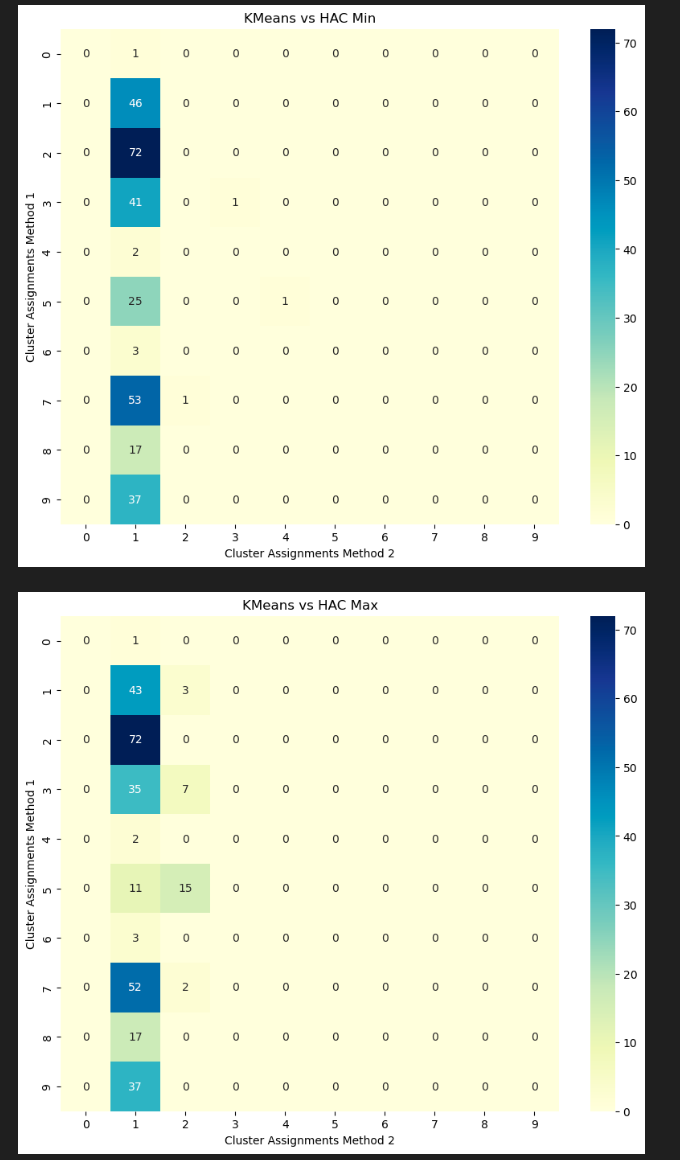
\includegraphics[width=0.5\linewidth]{hw4/25.png} \\ 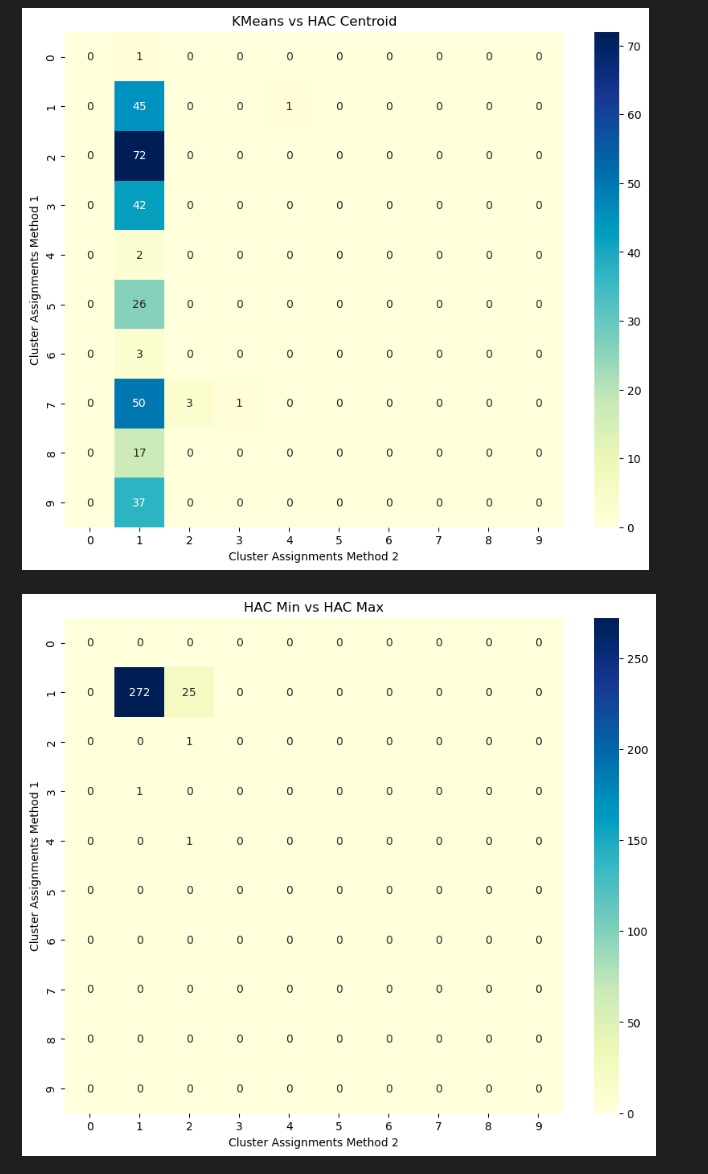
\includegraphics[width=0.5\linewidth]{hw4/26.png} \\ 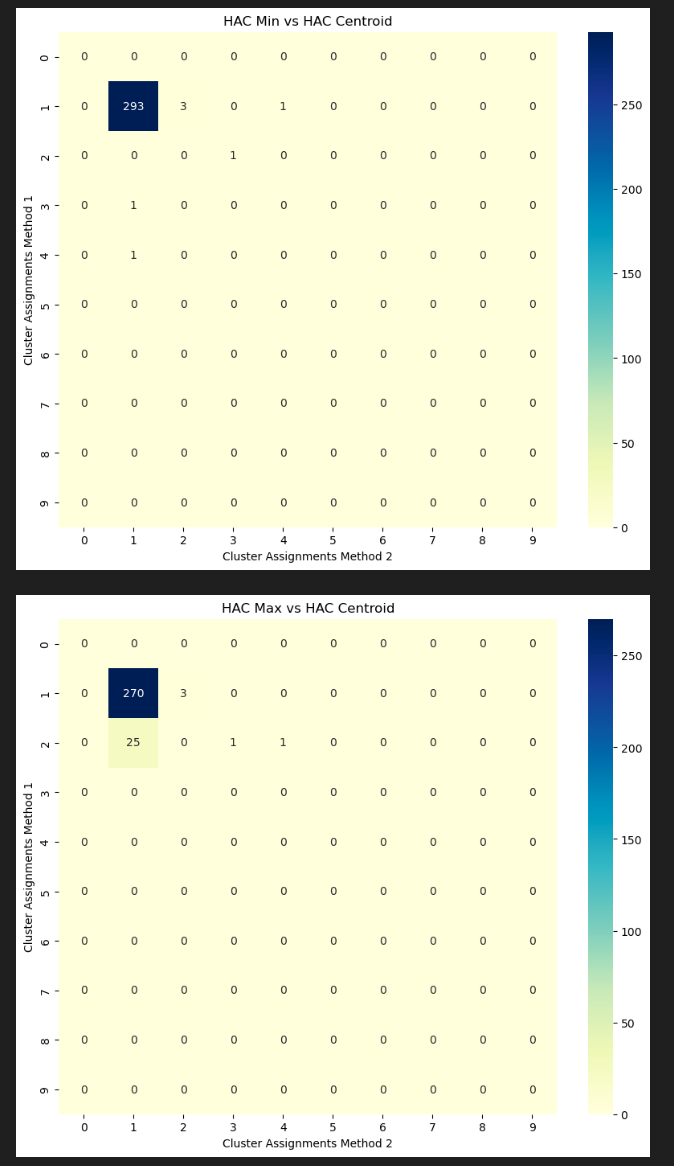
\includegraphics[width=0.5\linewidth]{hw4/27.png} \\ By looking at the diagonals of the confusion matrices as indicators of a high degree of agreement, I find that HAC Centroid has is the most similar to K-means. This is likely due to the centroid method in HAC making decisions based on the center of clusters, which is similar to how centroids are updated in K-means. \\
7.  (a) Clustering relies on the assumption that data points within the same group are more similar to each other than to those in other groups, which can be problematic for digit identification due to the high intra-class variability and inter-class similarity. Aligning clusters with labels presumes that each of the digit types forms a new group in the feature space, which is difficult to hold true in the case of the handwritten digits we work with. Clustering can thus generically be helpful, but may need supervised learning or labeling to be optimized. As such, clusters are incomplete without true labels, and without them the clusters don't represent meaningful classifications. \\
(b)  Clustering can be compromised by adding adversarial examples that are designed to lie near the decision boundary of clusters or within another cluster's domain, effectively causing misclassification. This is similar to what we saw with adversarial attacks on classifiers like kNN, which involve crafting inputs that are classified incorrectly due to their proximity to decision boundaries. Unlike kNN though where attacks are with respect to specific neighbors, attacks on targets change the overall data distribution. Generative classifiers model the entire distribution of each class and are misled by such examples that take advantage of learned distributions. Clustering is thus sensitive to the data's underlying structure. 
















 
\newpage


\newpage
%%%%%%%%%%%%%%%%%%%%%%%%%%%%%%%%%%%%%%%%%%%%%
% Problem 3
%%%%%%%%%%%%%%%%%%%%%%%%%%%%%%%%%%%%%%%%%%%%%

\begin{problem}[Ethics Assignment, 5pts]

Consider the simulation we conducted in class. There you were part of a health-care administration company, Optimizing Health. Optimizing Health is a small startup and you were a developer reporting directly to the CTO. In particular, you were responsible for designing a system that predicts the healthcare needs of an individual. First, you needed to choose a way to predict healthcare needs. You chose between approximating need by:

\begin{itemize}
    \item the predicted healthcare expenditure of that individual
    \item the predicted number of hours an individual is expected to visit the doctor’s office.
    \item the number of diagnoses the patient has received in the past year.
    \item the average prognosis for individuals in that patient’s age and racial groups.
\end{itemize}

As an organization, you settled on predicting healthcare need by predicted healthcare expenditure of that individual given their diagnosis.

Then, you used that predicted healthcare expenditure to assign a "Risk Score" to all patients, and, for patients above a certain cutoffs, you either automatically enrolled them in the a new program you created called the Medical Management Program (high risk) or referred them to their physician (moderate risk).

You discovered that, at a given Risk Score, Black patients are sicker than White patients. The algorithm was therefore less likely to recommend additional care to Black patients who needed it than White patients. 17.7$\%$ of Black patients were being recommended for additional care, while 46.5$\%$ of Black patients required additional care. After these recommendations were used, doctors provided disparate treatment, with Black patients not entering the Medical Management Program as frequently as they require.

All of these (and many unstated but salient) steps can be modeled using causal chains, backward looking responsibility, and forward looking responsibility (as we did in class).

After the terrible outcome, the CEO resigns and you are promoted to lead the organization! This means that any actions you take will be implemented and so you vow to do better. 

The first thing you do is decide to rewrite the mission: “Optimizing Health’s new mission is to provide care to individuals who need it but are not currently receiving it, without increasing healthcare disparities across groups.”

With this new goal in mind, think through each important choice-point for success and outline (literally draw) a new causal chain (similar to what you did in Scenario Part 4 in class). This time, however, you can recommend choices other than those outlined in the in-class Scenario and above. 

A sufficiently descriptive causal chain will include points that link the mission to, for instance, the choice to use ML, data collection, feature selection, ... , assignment of risk, what to do with risk scores, and so on. Remember to represent actual decision points as ovals and everything else (things that follow directly from decisions) as rectangles. Moreover, flag the decisions that carry moral or ethical responsibility to distinguish them from decisions that do not. At each point in the chain, if that point involves an ethically salient decision, provide your brief rationale for the decision, a brief description of the main argument against it, and your response to that objection. List the individuals who would be morally responsible at each contributing choice point. Finally, briefly describe how the outcome (the last node in your chain) meets the mission objective.


\end{problem}

\subsection*{Solution}

\newpage 

3.  I'm not sure how to draw a graph in latex, so instead of hand-drawing it or using an alternative source I will label the following criteria according to what we discussed in class. 

The updated mission emphasizes providing care to individuals in need, especially those currently underserved, while actively working to reduce healthcare disparities. The causal chain and decision-making process uses data collection, feature selection, risk assessment, and intervention strategies. 
\newline

Step 1: Re-evaluating the Use of ML in Healthcare Prediction

**Decision Point (Oval):** Choice to continue using ML for healthcare predictions.

- Ethical Rationale: ML can efficiently process vast amounts of data to identify at-risk individuals, potentially uncovering nuanced patterns not visible to humans.
- Main Ethical Concern: Risk of perpetuating existing biases in the data, leading to unequal healthcare recommendations.
- Response: Implement rigorous bias detection and mitigation techniques at every stage of the ML pipeline.
- Moral Responsibility: Data scientists and ethicists must collaborate to ensure the algorithm's fairness. 
\newline

Step 2: Data Collection and Feature Selection

**Decision Point (Oval):** Determining which data points and features to include.

- Ethical Rationale: Inclusive and diverse data collection can help understand varied healthcare needs across different demographics.
- Main Ethical Concern: Poor training can result in over-reliance on sensitive attributes (e.g., race, age). This will just reinforce stereotypes or lead to discrimination.
- Response: Use demographic data responsibly to identify and correct disparities, not to make decisions based solely on these attributes.
- Moral Responsibility: Data engineers and ethicists are responsible for ethical data collection and feature selection practices.
\newline 

Step 3: Definition and Assignment of Risk Scores

**Decision Point (Oval):** How to calculate and utilize risk scores.

- Ethical Rationale: Risk scores should accurately reflect individuals' healthcare needs to allocate resources efficiently and equitably.
- Main Ethical Concern: A single-dimensional risk score (e.g., predicted expenditure) might not capture the complexity of healthcare needs. I will created a weighted system using different resource optimization to measure this. 
- Response: Develop a multidimensional risk score that includes expenditure, doctor visits, diagnosis history, family history, and tailored metrics for underserved groups.
- Moral Responsibility: ML developers and healthcare professionals need to ensure that risk scores are comprehensive and equitable.
\newline 

Step 4: Intervention Strategies Based on Risk Scores

**Decision Point (Oval):** Deciding on interventions for different risk levels.

- Ethical Rationale: Targeted interventions can help direct resources where they are most needed, especially to underserved populations. My ML research in high school focused on how to best target underserved populations to maximize treatment-adjusted mortality disparities, so this would be the focus of this section. 
- Main Ethical Concern: There's a risk of resource misallocation if interventions are not carefully designed and implemented.
- Response: Continuous evaluation and adjustment of intervention thresholds and strategies based on outcome data and feedback from healthcare professionals and patients.
- Moral Responsibility: Healthcare administrators and policy makers are responsible for the ethical allocation of interventions.
\newline

Step 5: Outcome - Achieving the Mission
**Outcome (Rectangle):** Reduced healthcare disparities and improved access to necessary care for underserved individuals.

- Ethical Rationale: The updated rationale aims to identify and address the healthcare needs of all individuals, with special attention to historically underserved groups, thereby reducing disparities.
- Moral Responsibility: The entire organization, led by the new CEO, is responsible for ensuring the mission's success through ethical decision-making, implementation, and continuous improvement.
\newline

Net Diagram: 

As described, the causal chain shows how agents in healthcare may decide to use ML by properly aggregating data and selecting features, with the goal of ultimately reducing healthcare disparities and improving access to care. I use the same metrics as earlier with decision points marked as ovals, outcomes as rectangles, and ethical considerations highlighted at each decision point.

\newpage
%%%%%%%%%%%%%%%%%%%%%%%%%%%%%%%%%%%%%%%%%%%%%
% Name and Calibration
%%%%%%%%%%%%%%%%%%%%%%%%%%%%%%%%%%%%%%%%%%%%%
\subsection*{Shreshth Rajan}

\subsection*{Collaborators and Resources}
Whom did you work with, and did you use any resources beyond cs181-textbook and your notes? I used only the textbook, OH, and course staff. 

\end{document}
